\begin{frame}
\frametitle{Argo}
% in documenet
\begin{columns}
\column{0.5\textwidth}
\begin{figure}
    \centering
    \begin{minipage}{.9\columnwidth}
    \includegraphics[width=\linewidth]{floats-together.png}
    \caption{\tiny{APEX float (left). Image taken from \url{http://argofloats.wikispaces.com/home} Deep Solo prototype (right) Taken by me at SIO.}}
    \end{minipage}
\end{figure}
\column{0.5\textwidth}
\begin{figure}
    \vspace*{-.73cm}
    \centering
    \begin{minipage}{.9\columnwidth}
    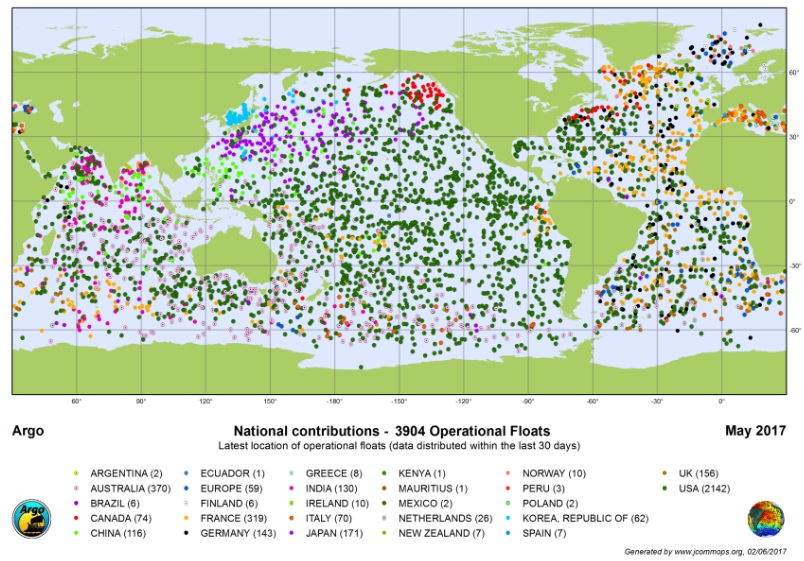
\includegraphics[width=\linewidth]{Argo-Floats-May-2017.jpg}
    \caption{\tiny{Image taken from \url{http://argofloats.wikispaces.com/home}}}
    \end{minipage}
\end{figure}
\vspace*{-.4cm}
\underline{\textbf{Research topics}}
\begin{itemize}
    \item How to access data?
    \item How to visualize data set?
    \item How to handle errors?
\end{itemize}
\end{columns}
\end{frame}

\begin{frame}
\frametitle{Argo Terminology}
\begin{itemize}
    \item Profile: Prray of measurements taken by float/platform.
    \item Platform: Device that takes profiles. Platform $\equiv$ Float.
    \item Selection: Profiles grouped by area, date, depth, etc.
\end{itemize}
\end{frame}

\begin{frame}
\frametitle{Coriolis Visualization Application}
\begin{columns}
\column{0.65\textwidth}
\begin{figure}
\begin{minipage}{1\columnwidth}
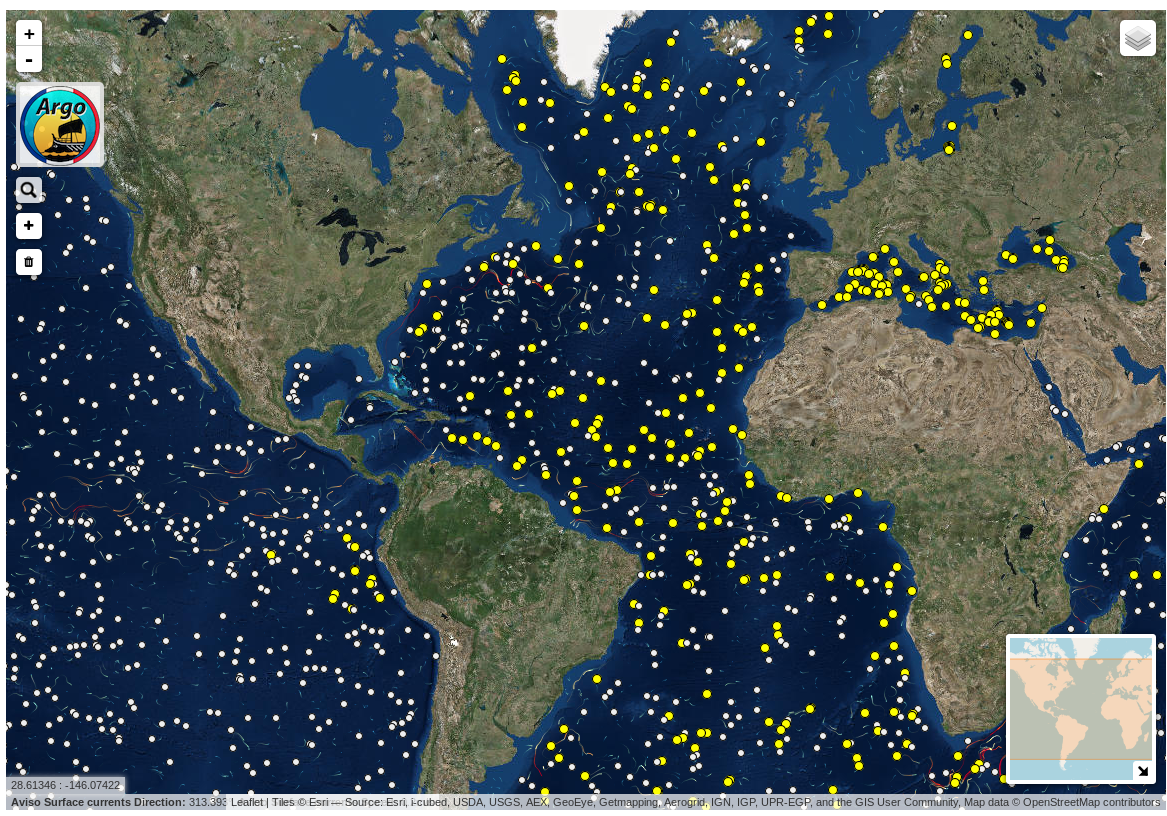
\includegraphics[width=.5\linewidth]{argo_france.png}
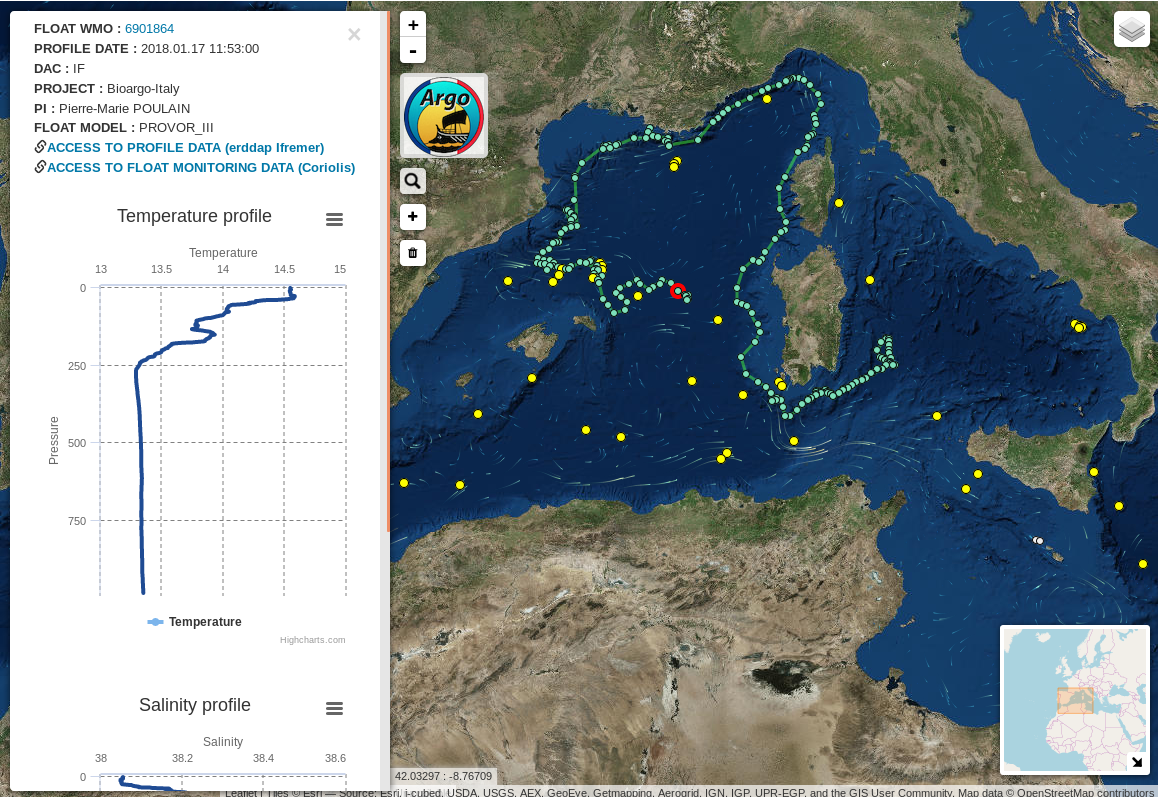
\includegraphics[width=.5\linewidth]{argo_france_zoomed.png}
\caption{\tiny{Argo Active network map (left) \url{http://www.argo-france.fr/en/argo-active-network-map/}Showing argo profiles owned by the Coriolis (French) DAC. Yellow dots represent floats operated by the Coriolis project. Selecting a dot reveals a side panel with additional information (right). Velocity field animations overlay the profile dots showing currents generated via ANDRO. Screenshot taken from \url{http://map.argo-france.fr/}}}
\end{minipage}
\end{figure}
\column{.35\textwidth}
\small{\underline{\textbf{Pros:}}}
\begin{itemize}
    \item Fast
    \item Intuitive
    \item Interactive
\end{itemize}
\small{\underline{\textbf{Cons:}}}
\begin{itemize}
    \item Can't select regions
    \item Can't select platforms
    \item Limited to recent profiles
    \item Highcharts aren't FOSS
\end{itemize}
\end{columns}
\end{frame}

\begin{frame}
\frametitle{NASA Sea Level Change Data Analysis Tool}
\begin{columns}
\column{0.65\textwidth}
\begin{figure}
\begin{minipage}{1\columnwidth}
\centering
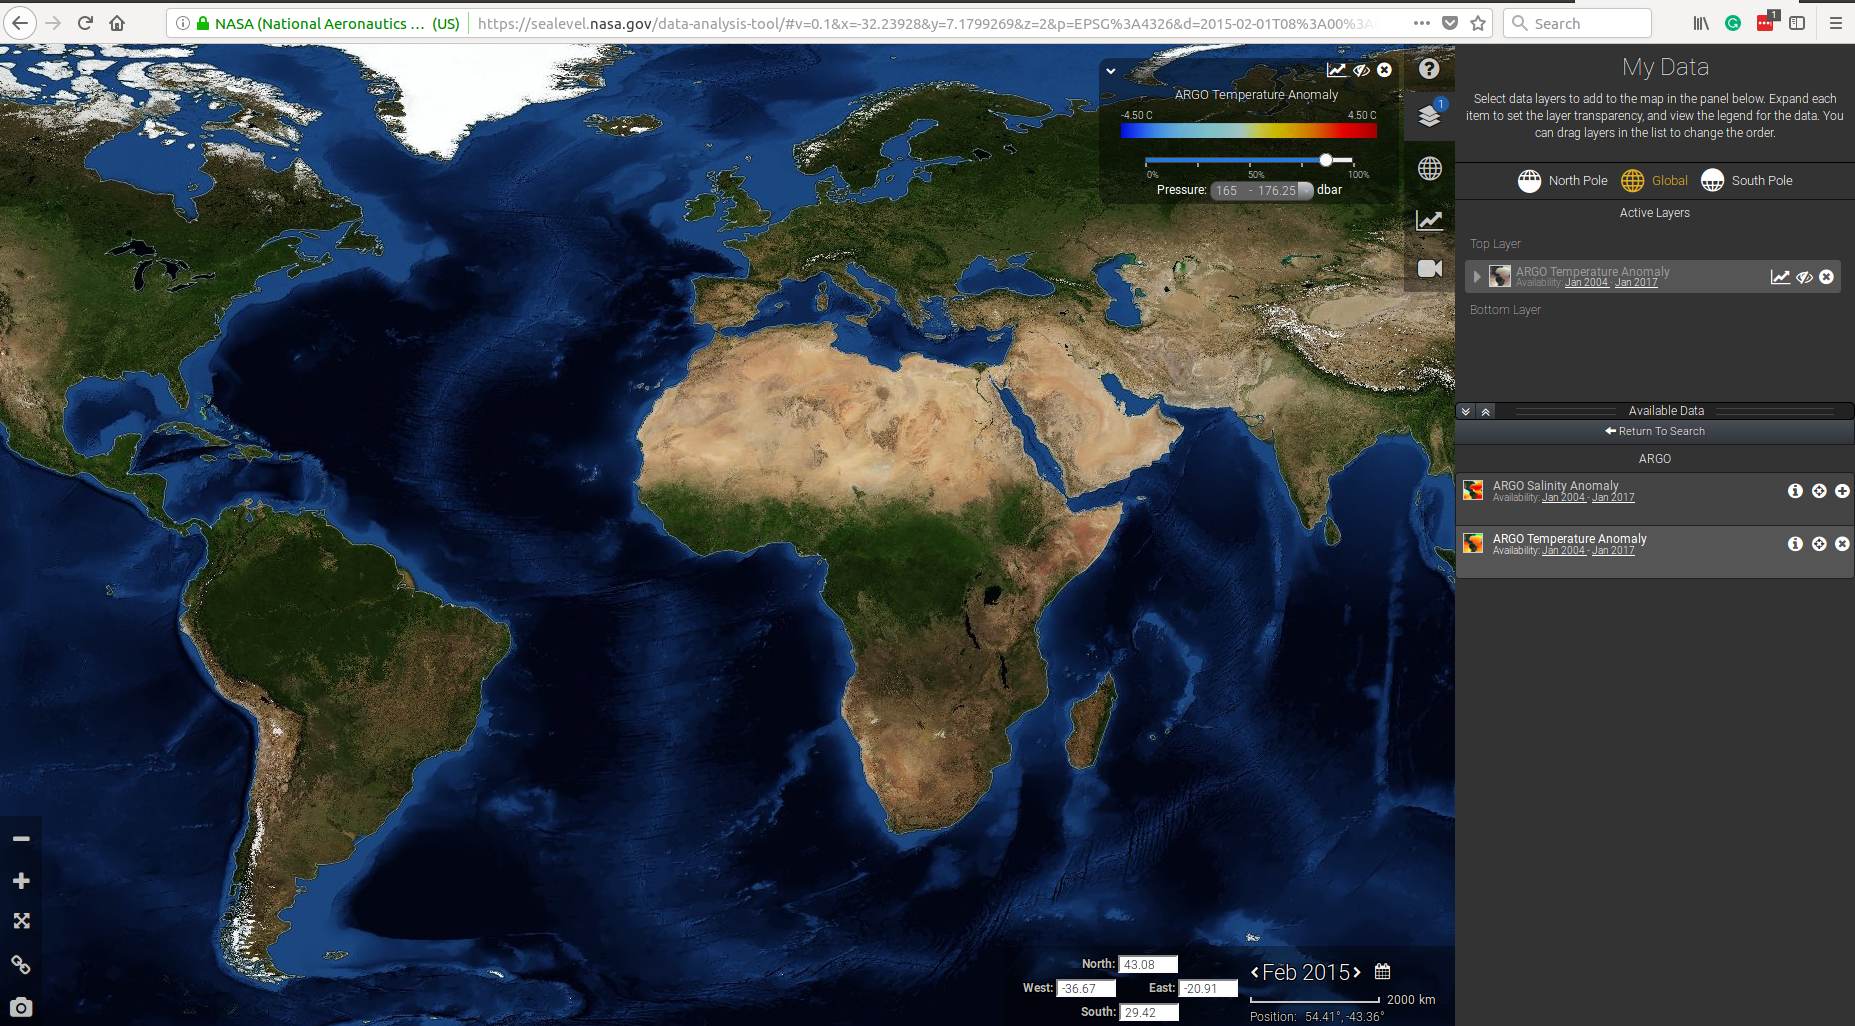
\includegraphics[width=\linewidth]{datMain.png}
\caption{\tiny{DAT web app format with Data tab displayed on the side bar. Argo derived gridded salinity and temperature products from January 2004 to January 2017 are available to plot. Screenshot taken from \url{https://sealevel.nasa.gov/data-analysis-tool/}}}
\end{minipage}
\end{figure}
\column{0.35\textwidth}
\small{\underline{\textbf{Pros:}}}
\begin{itemize}
    \item Regional selection
    \item Offers several data sets
    \item Time series
    \item Contour images overlay
\end{itemize}
\small{\underline{\textbf{Cons:}}}
\begin{itemize}
    \item Cuts off in middle of ocean
    \item Slow
    \item Non-intuitive
    \item Beta product (includes bugs)
    \item Limited to gridded products
\end{itemize}
\end{columns}
\end{frame}

\begin{frame}
\frametitle{4D Visual Delivery of Big Climate Data: MrSharky}
\begin{columns}
\column{0.5\textwidth}
\begin{figure}
\vspace*{-.6cm}
\begin{minipage}{1\columnwidth}
\centering
\fbox{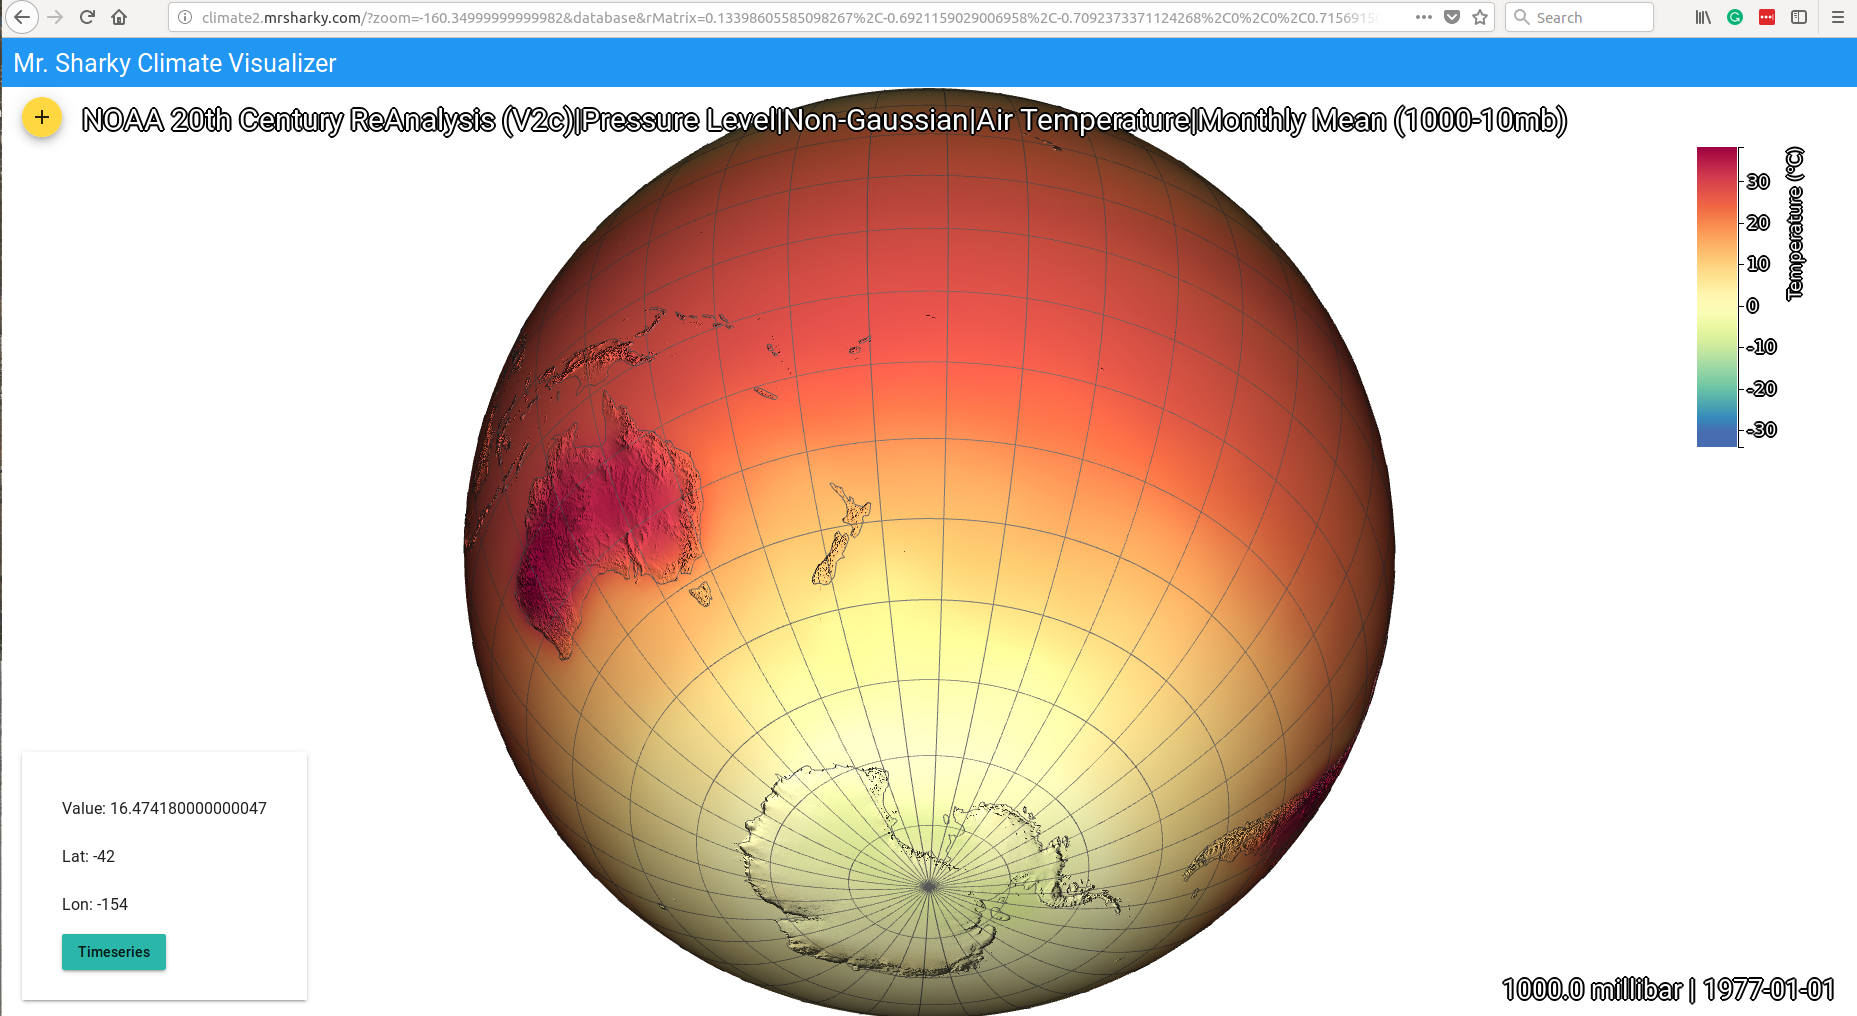
\includegraphics[width=.75\linewidth]{mrSharkySouthView.png}}
\fbox{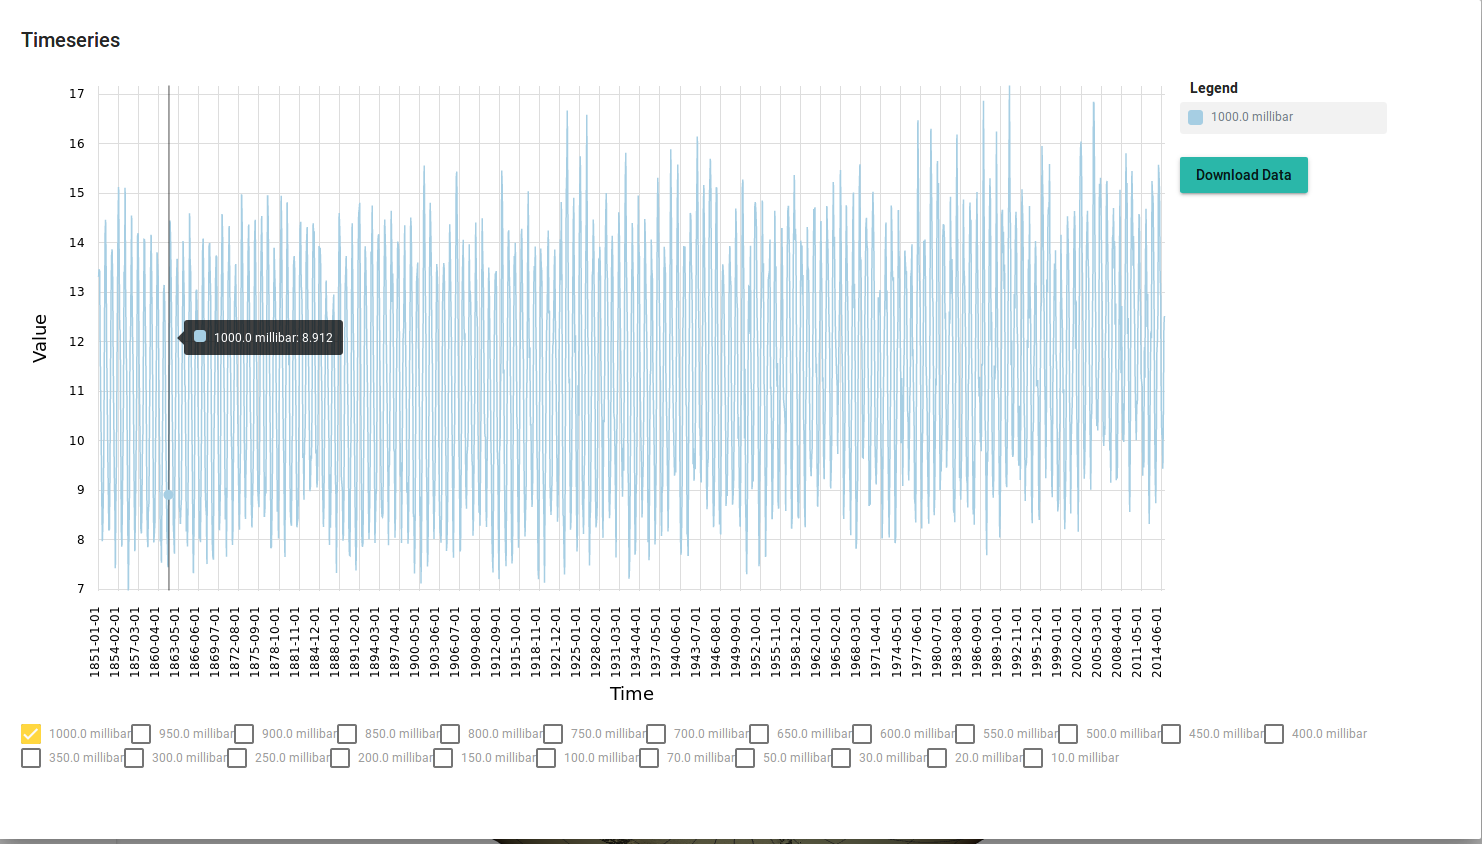
\includegraphics[width=.75\linewidth]{mrShTS.png}}
\caption{\tiny{Clicking a point on the globe will generate a box element showing the point's value and latitude-longitude coordinates, shown in the lower left corner of the (top) subfigure. Clicking the teal button will generate a time series (bottom) that can be downloaded as a .csv file. Screenshots taken from \url{http://climate2.mrsharky.com/}}}
\end{minipage}
\end{figure}
\column{0.35\textwidth}
\small{\underline{\textbf{Pros:}}}
\begin{itemize}
    \item Rich with custom viewing features
    \item View in seveal projections
    \item Provides time series
    \item Uses several products
\end{itemize}
\small{\underline{\textbf{Cons:}}}
\begin{itemize}
    \item Resource heavy
    \item Little documentation on how to use
    \item Limited chart capability
    \item Limited to gridded products
\end{itemize}
\end{columns}
\end{frame}

\begin{frame}
\frametitle{Visualization and Data Retrieval Tool: Argovis}
\begin{columns}
\column{0.5\textwidth}
\begin{figure}
\vspace*{-.6cm}
\begin{minipage}{1\columnwidth}
\centering
\fbox{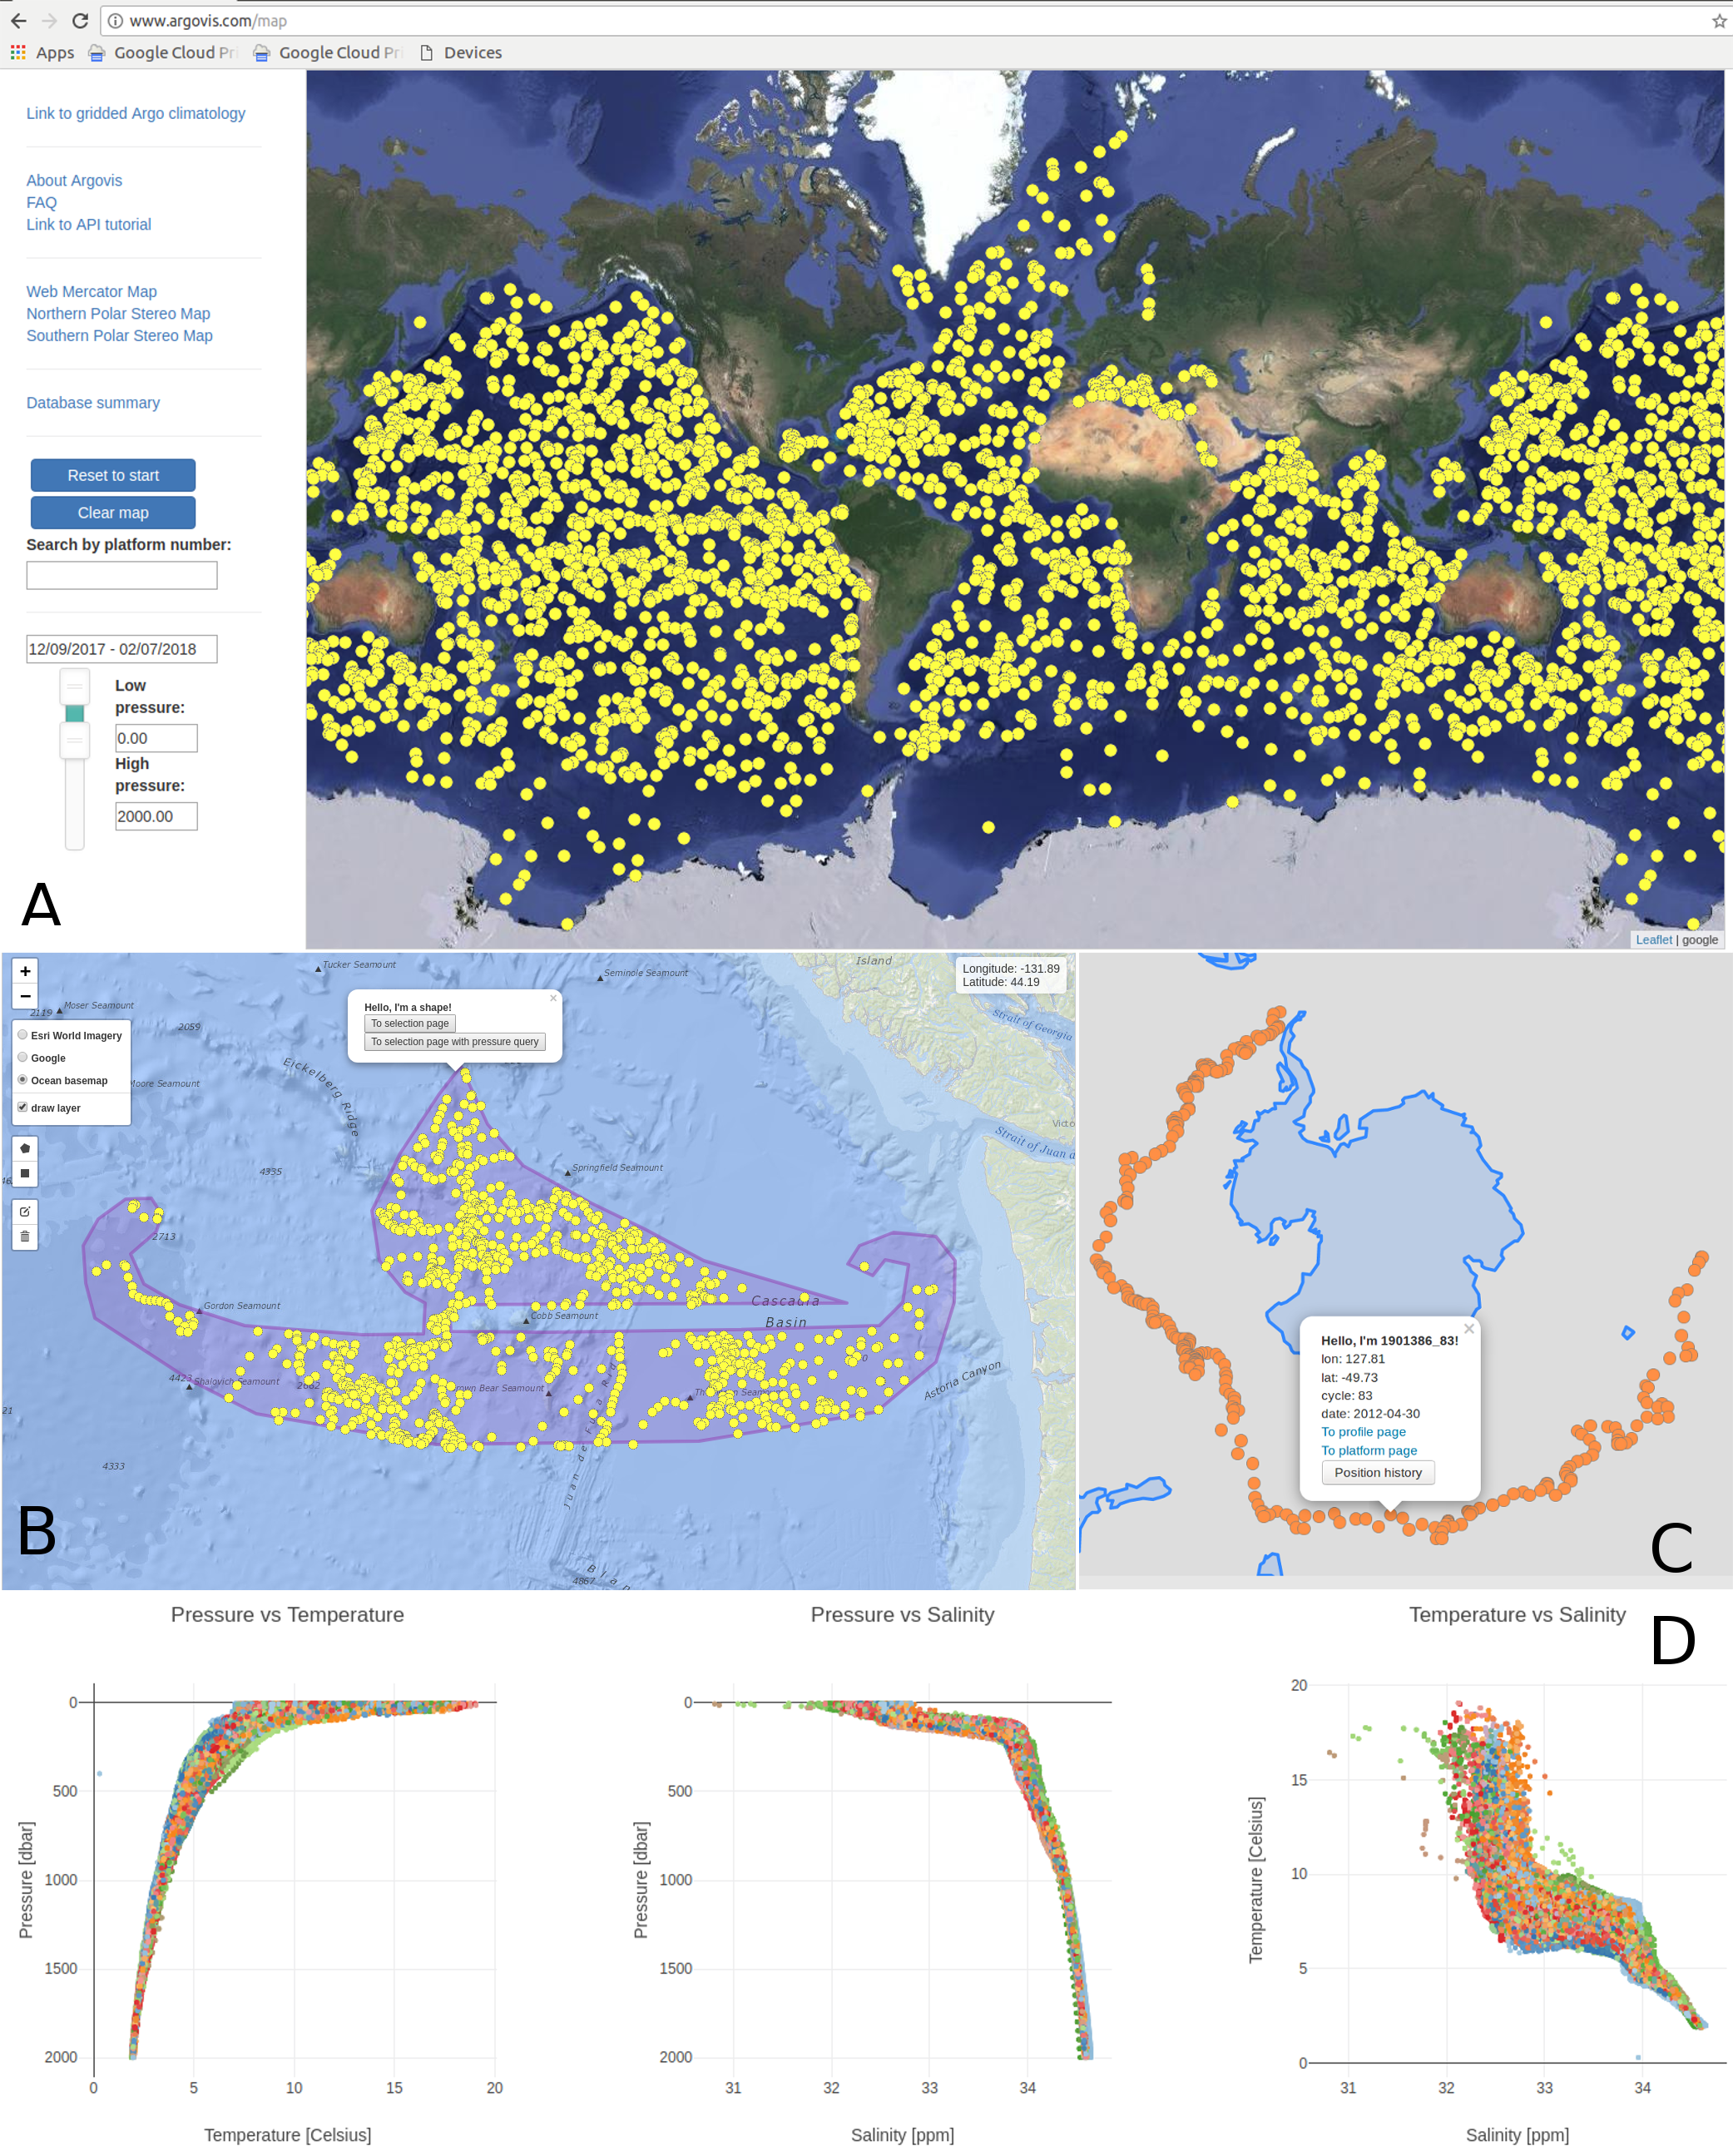
\includegraphics[width=.75\linewidth]{mainFig.png}}
\caption{\tiny{Argovis features: interactive map (top) Selection(mid right), stereo projection (left), data charts (bottom)}}
\end{minipage}
\end{figure}
\column{0.35\textwidth}
\small{\underline{\textbf{Pros:}}}
\begin{itemize}
    \item Custom viewing features
    \item Includes stereographic projection
    \item Interactive map
    \item API included
    \item Video tutorials! \url{https://www.youtube.com/watch?v=IlNJ0owuTHM}
\end{itemize}
\small{\underline{\textbf{Cons:}}}
\begin{itemize}
    \item No time series
    \item Only Argo data
    \item No gridded products
\end{itemize}
\end{columns}
\end{frame}



\begin{frame}
\frametitle{Argo Data}
\begin{figure}
\centering
\begin{minipage}{1\columnwidth}
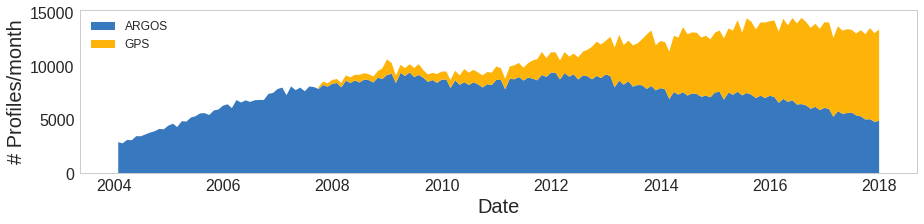
\includegraphics[width=\linewidth]{psTS.png}
\caption{History of Argo profiles reported each month since the programs in-
ception. Trends towards GPS measurements indicate a need for a data retrival service. Argo data generation is increasing in the number of profiles reported and by the
amount of data reported by each profile.}
\end{minipage}
\end{figure}
\end{frame}

\begin{frame}
\frametitle{Argo FTP}
\begin{figure}
\centering
\begin{minipage}{1\columnwidth}
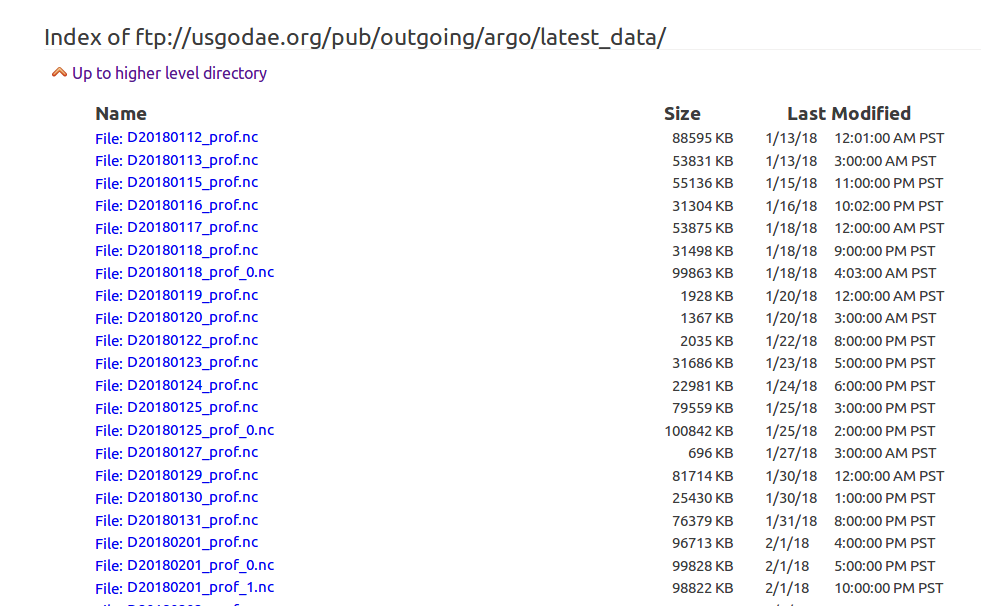
\includegraphics[width=\linewidth]{argo-ftp.png}
\caption{Screenshot of FTP data retrieval taken from \url{ftp://usgodae.org/pub/outgoing/argo/latest_data/}}
\end{minipage}
\end{figure}
\end{frame}

% I wrote a webapp that takes ftp data and puts it in a mongo database.

% website overview

% show video tutorial

% database is interfaced by express.js

% html Pages are served by express.js. Serves json or html. access is centered around the url.

% data only flows out, no destroying or creating data (by app)

% FTP to JSON converter is in python. Show algorithm
\begin{frame}[fragile]
\frametitle{Argovis JSON output}
\begin{lstlisting}[language=JavaScript, basicstyle=\tiny, caption=JSON schema of mongoDB profile.]
{
  "_id": <String>,
  "max_pres": <Int>,
  "measurements": <List[{temp: <Number>,
                         psal: <Number>,
                         pres: <Number>,
                         ...}]>,
  "date": <ISODate>,
  "POSITIONING_SYSTEM": <String>,
  "PLATFORM_TYPE": <String>,
  "DATA_MODE": <String>,
  "PI_NAME": <String>,
  "cycle_number": <Int>,
  "lat", <Number>,
  "lon", <Number>,
  "geoLocation", {"type": "Point",
                  "coordinates": [<Number[2]>],
  "dac": <String>,
  "platform_number": <String>,
  "station_parameters": <List[String]>, 
  "nc_url": <String>
}
\end{lstlisting}
\end{frame}

% Python API. Show the 3 main functions
\begin{frame}[fragile]
\frametitle{API: Profile function}
\begin{lstlisting}[basicstyle=\tiny, caption=Python function to retrieve profile data. Uses 'requests' library]
def get_profile(profile_number):
    resp = requests.get('http://www.argovis.com/catalog/profiles/'+profile_number)
    # Consider any status other than 2xx an error
    if not resp.status_code // 100 == 2:
        return "Error: Unexpected response {}".format(resp)
    profile = resp.json()
    return profile
\end{lstlisting}
\end{frame}

\begin{frame}[fragile]
\frametitle{API: Platform function}
\begin{lstlisting}[basicstyle=\tiny, caption=Python function to retrieve platform data]
def get_platform_profiles(platform_number):
    resp = requests.get('http://www.argovis.com/catalog/platforms/'+platform_number)
    # Consider any status other than 2xx an error
    if not resp.status_code // 100 == 2:
        return "Error: Unexpected response {}".format(resp)
    if resp.status_code == 500:
        return "Error: 500 status {}".format(resp)
    platformProfiles = resp.json()
    return platformProfiles
\end{lstlisting}
\end{frame}

\begin{frame}[fragile]
\frametitle{API: Selection function}
\begin{lstlisting}[basicstyle=\tiny, caption=Python function to retrieve selection data]
def get_selection_profiles(startDate, endDate, shape, presRange=None):
    baseURL = 'http://www.argovis.com/selection/profiles'
    startDateQuery = '?startDate=' + startDate
    endDateQuery = '&endDate=' + endDate
    shapeQuery = '&shape='+shape.replace(' ','')
    if not presRange == None:
        pressRangeQuery = '&presRange=' + presRange
        url = baseURL + startDateQuery + endDateQuery + pressRangeQuery + shapeQuery
    else:
        url = baseURL + startDateQuery + endDateQuery + shapeQuery
    resp = requests.get(url)
    # Consider any status other than 2xx an error
    if not resp.status_code // 100 == 2:
        return "Error: Unexpected response {}".format(resp)
    if resp.status_code == 500:
        pdb.set_trace()
        return "Error: 500 status {}".format(resp)
    selectionProfiles = resp.json()
    return selectionProfiles
\end{lstlisting}
\end{frame}


% Applications. Time series, meta plots, contour plots, histograms
\begin{frame}
\frametitle{API: Time Series Applications}
\begin{figure}
\centering
\begin{minipage}{.8\columnwidth}
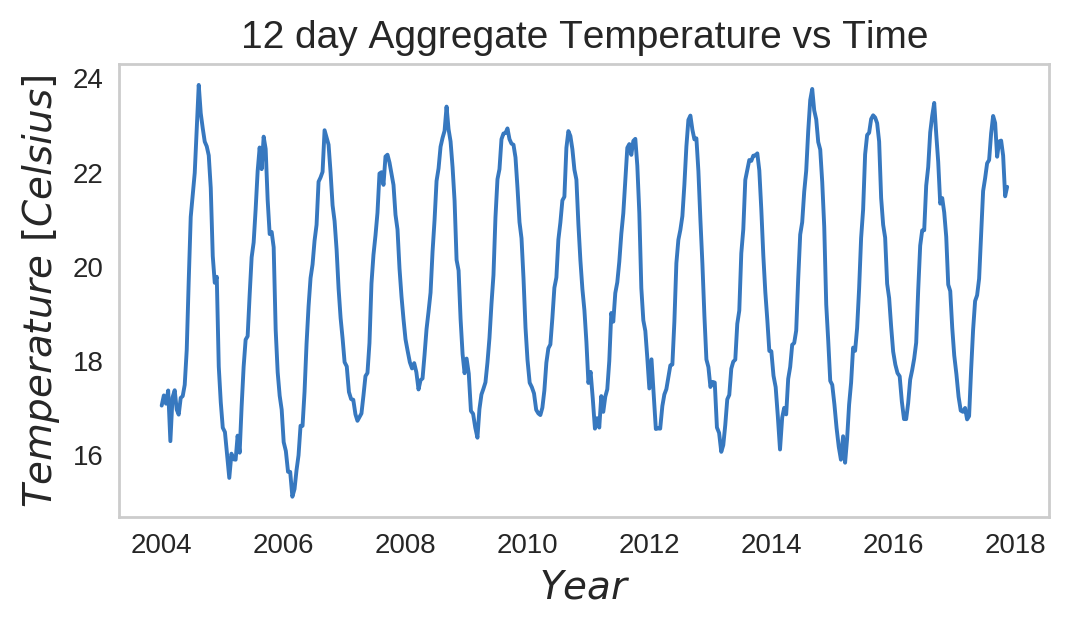
\includegraphics[width=\linewidth]{ts.png}
\caption{API includes a special time series generator for a selection.}
\end{minipage}
\end{figure}
\end{frame}

% Applications. Time series, meta plots, contour plots, histograms
\begin{frame}
\frametitle{API: Time Series Applications}
\begin{figure}
\centering
\begin{minipage}{.65\columnwidth}
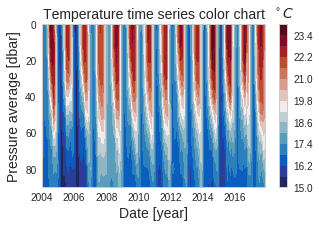
\includegraphics[width=1\linewidth]{tempColorChart.png}
\caption{Time series at ten equally spaced partitions along the first 100 meters of the water column (10 meters/partition). Temperature is displayed as color and the y-axis is plotted as pressure (depth).}
\end{minipage}
\end{figure}
\end{frame}

\begin{frame}
\frametitle{API: Histogram on Basemap}
\begin{figure}
\centering
\begin{minipage}{1\columnwidth}
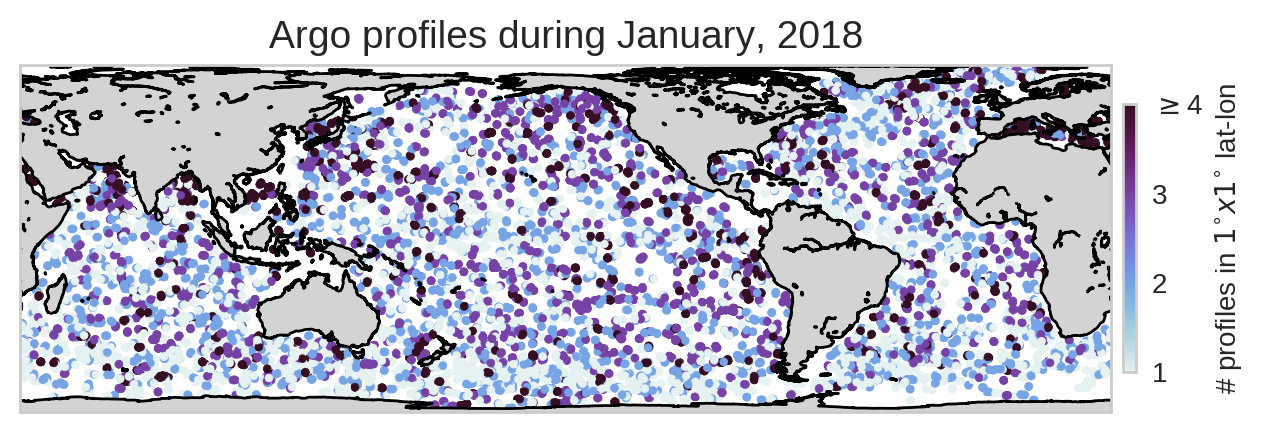
\includegraphics[width=1\linewidth]{worldHist.png}
\caption{SST time series of selection. Color chart was made using a cubic interpolation of 10 different depths aggregated every 10 dbar.}
\end{minipage}
\end{figure}
\end{frame}

\begin{frame}
\frametitle{API: View Float Types}
\begin{figure}
\centering
\begin{minipage}{1\columnwidth}
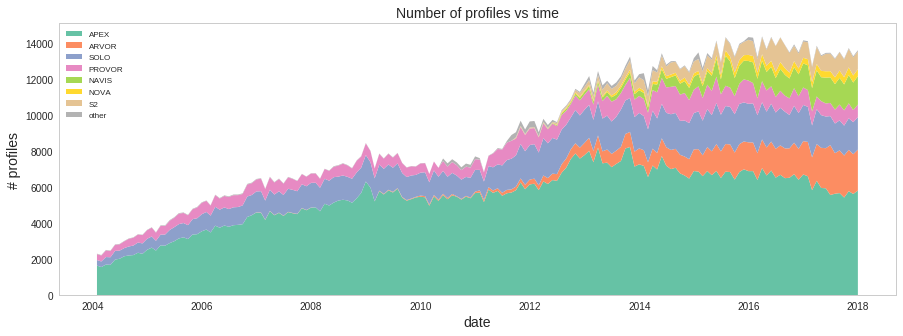
\includegraphics[width=1\linewidth]{typeTS.png}
\caption{Number of profiles reported per month vs Time.}
\end{minipage}
\end{figure}
\end{frame}

\begin{frame}
\frametitle{Next Steps}
\begin{itemize}
    \item Create Kaggle.com competition using Argovis.com's database
    \item Include API in other languages, (R, MATLAB, Julia, etc.)
    \item Publish website release in a scientific journal
    \item Apply for a research grant for further development/testing.
    \item Included a gridded product section to the website.
\end{itemize}
\end{frame}